% =============================================================
%  SECTION: Module 6 — Radial Distribution Function
%  ASSIGNED TO: [Person Name]
%
%  GUIDING QUESTIONS TO ANSWER:
%   WHAT  — What is g(r)? What does it measure physically?
%   WHY   — Why can't temperature alone tell us if a system is solid or liquid?
%           Why must we normalise by the shell volume and density?
%           Why must g(r) → 1.0 at large r?
%   HOW   — How is the histogram binned? How is the normalization applied?
%           What is the MIC used for in this context?
%  EXTRAS — What do sharp peaks vs. broad/decaying peaks mean physically?
%           Statistical binning: why average over multiple frames?
% =============================================================

\newpage
\section{Module 6: Radial Distribution Function}

\subsection{What Are We Doing?}
% We need a structural metric to distinguish solid from liquid.
% g(r) gives the probability of finding an atom at distance r from a central atom,
% relative to a uniform ideal gas.
% [WRITE HERE]

\subsection{Why Are We Doing It?}

\subsubsection{Why Isn't Temperature Enough?}
% A glass and a liquid can be at the same temperature.
% Structure (how atoms are arranged) is distinct from thermodynamics.
% We need to look at the spatial correlations between atoms.
% [WRITE HERE — build intuition]

\subsubsection{Why Does \texorpdfstring{$g(r) \to 1$}{g(r)→1} at Large \texorpdfstring{$r$}{r}?}
% At large distances, correlations die out. The probability of finding an atom
% is just the bulk density. Dividing by the ideal gas density gives 1.0.
% If g(r) doesn't reach 1.0, the normalization or the simulation is wrong.
% [WRITE HERE]

\subsubsection{What Do the Peaks Tell Us?}

\begin{description}
    \item[Solid:] Sharp, narrow peaks at well-defined distances corresponding to the coordination shells of the FCC lattice. Long-range order persists.
    \item[Liquid:] A prominent first peak (nearest-neighbour shell), then broad, decaying oscillations that quickly reach 1.0, indicating short-range order only.
\end{description}

% [ADD PHYSICAL INTUITION — what is the first peak? second peak?]

\subsection{How Is It Implemented?}

\subsubsection{Algorithm}

\begin{equation}
    g(r) = \frac{V}{4\pi r^2 \Delta r \, N^2}
    \left\langle \sum_i \sum_{j \neq i} \mathbf{1}\!\left[r < r_{ij} < r + \Delta r\right] \right\rangle
    \label{eq:gr}
\end{equation}

\begin{enumerate}
    \item For each snapshot, loop over all unique pairs $(i,j)$ and compute $r_{ij}$ using the MIC.
    \item Bin each $r_{ij}$ into a histogram with bin width $\Delta r$ and up to $r_{\max} = L/2$.
    \item Normalise each bin $k$ (centre $r_k$) by the shell volume and number density:
    \begin{equation}
        g(r_k) = \frac{2 \cdot \text{count}(k) \cdot L^3}{N^2 \cdot 4\pi r_k^2 \Delta r}
        \label{eq:gr_norm}
    \end{equation}
    \item Average $g(r)$ over multiple uncorrelated snapshots from the production run.
\end{enumerate}

\subsubsection{Binning for Statistical Reliability}

Because consecutive MD timesteps are highly correlated, $g(r)$ is collected every 10 steps and the results are averaged. This reduces noise without requiring prohibitively long runs.

\subsection{Test Results}

% Test on a snapshot from the production run.
% Confirm: g(r) → 1.0 at large r (normalization correct).
% Confirm: first peak is near the LJ minimum at r* ≈ 1.12.

\begin{figure}[H]
    \centering
    % 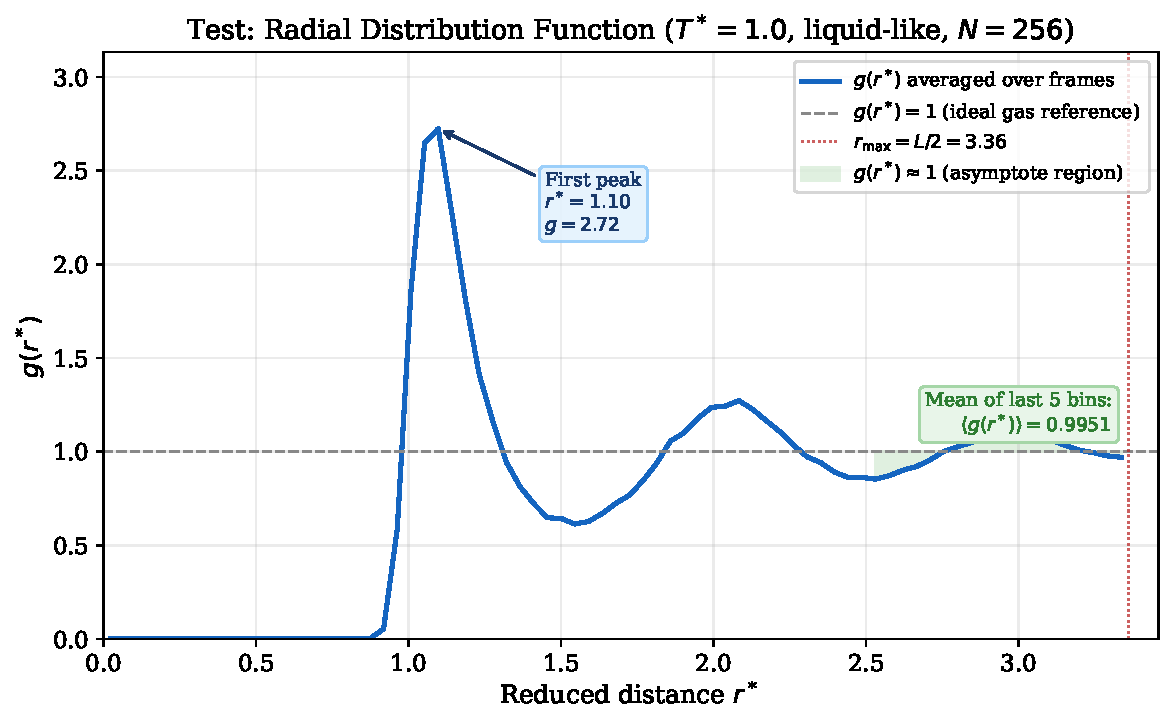
\includegraphics[width=0.75\linewidth]{figures/m6_gr_test.pdf}
    \caption{Test $g(r)$ plot from Module 6, computed on a single production snapshot. The function asymptotes to $g(r) = 1$ (dashed line) at large $r$, confirming correct normalisation.}
    \label{fig:m6_gr_test}
\end{figure}

% [WRITE DISCUSSION OF TEST RESULTS HERE]
